\subsection{Inteligencia Artficial}
Definir la Inteligencia Artificial puede resultar complejo, ya que la inteligencia misma es difícil de precisar. Algunas figuras prominentes la vinculaban con la ambición, mientras que otros la asociaban con la imaginación como motor fundamental, o con la capacidad de adaptarse a los cambios. Estas diversas definiciones sugieren que no existe un acuerdo claro sobre qué constituye la inteligencia, y aún menos sobre qué es la Inteligencia Artificial. No obstante, en términos generales, se puede entender por "Inteligencia Artificial" a cualquier sistema artificial que exhiba un comportamiento que pueda considerarse "inteligente". Esto incluye sistemas que imitan funciones sensoriales humanas, como la visión o la audición, así como aquellos capaces de aprender de manera autónoma según las necesidades de su entorno. \parencite{bk_hurbans2020grokking}


\subsection{Machine Learning}
El Aprendizaje Automático, también conocido como Machine Learning, se entiende como una disciplina que combina ciencia y arte, en la cual se le enseña a una computadora a aprender de manera autónoma a partir de los datos que se le proporcionan. \parencite{bk_geron2022handml}

En la Figura \ref{2:fig209} se presenta el enfoque tradicional del Machine Learning.

\begin{figure}[H]
	\begin{center}
		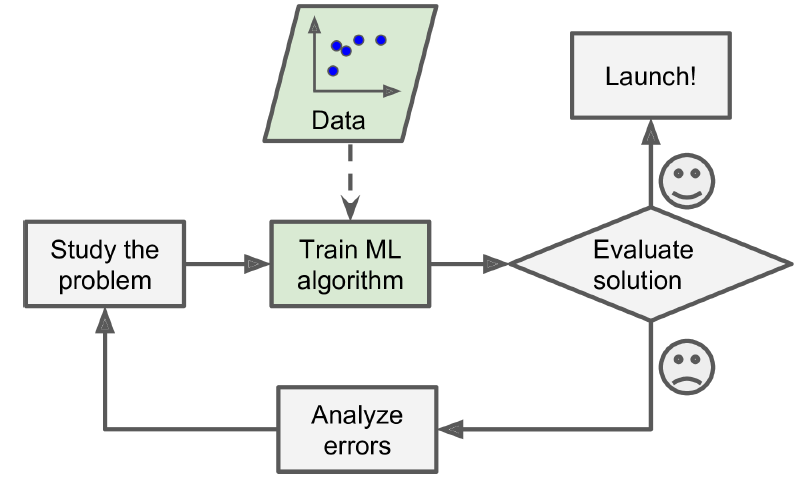
\includegraphics[width=0.75\textwidth]{2/figures/enfoque_ml.png}
		\caption[Enfoque del Machine Learning]{Enfoque del Machine Learning. \\
		Fuente: \cite{bk_geron2022handml}. \textit{Hands-on machine learning with Scikit-Learn, Keras, and TensorFlow}.}
		\label{2:fig209}
	\end{center}
\end{figure}



\subsection{Perceptrón}
Inventado por Frank Rosenblatt en 1957, el Perceptrón es la unidad básica de una red neuronal e incluso es considerado como la más simple red neuronal artificial (ANN). \parencite{bk_geron2022handml}

El Perceptrón se muestra en la Figura \ref{2:fig207-2}.

\begin{figure}[H]
	\begin{center}
		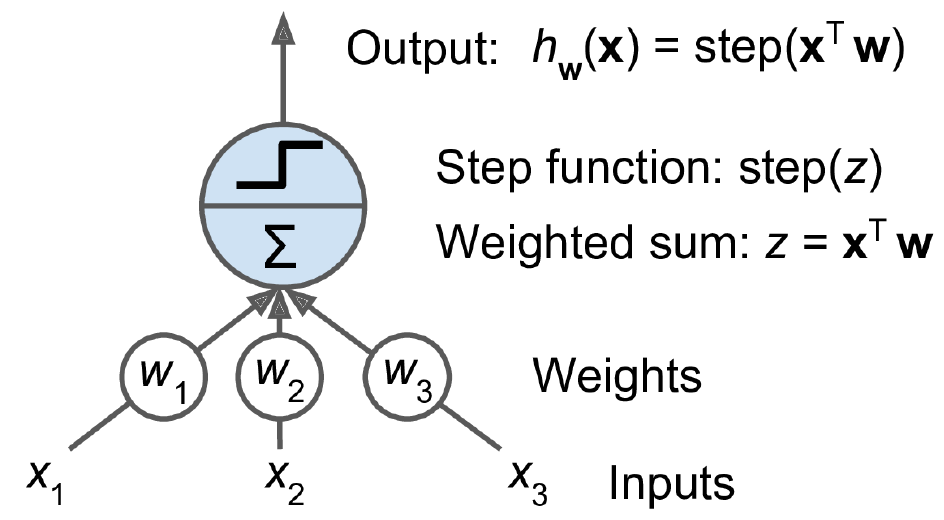
\includegraphics[width=0.75\textwidth]{2/figures/perceptron.png}
		\caption[Perceptrón]{Perceptrón. \\
		Fuente: \cite{bk_geron2022handml}. \textit{Hands-on machine learning with Scikit-Learn, Keras, and TensorFlow}.}
		\label{2:fig207-2}
	\end{center}
\end{figure}


\subsection{Perceptrón Multicapa}
Un Perceptrón Multicapa (MLP) se compone de múltiples perceptrones organizados en capas. Incluye una capa de entrada y una capa de salida, y todas las capas, excepto la de salida, contienen una neurona adicional conocida como bias \parencite{bk_geron2022handml}

Una representación gráfica de un MLP se muestra en la Figura \ref{2:fig208}.

\begin{figure}[H]
	\begin{center}
		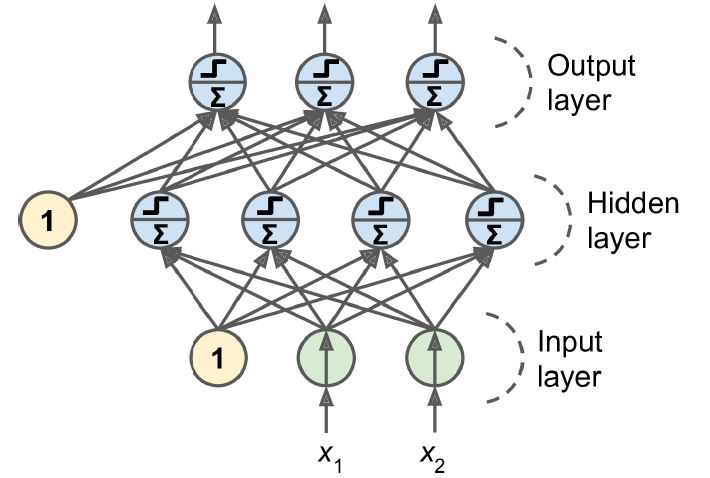
\includegraphics[width=0.77\textwidth]{2/figures/mlp.png}
		\caption[Perceptrón Multicapa]{Perceptrón Multicapa. \\
		Fuente: \cite{bk_geron2022handml}. \textit{Hands-on machine learning with Scikit-Learn, Keras, and TensorFlow}.}
		\label{2:fig208}
	\end{center}
\end{figure}



\subsection{Redes Neuronales Convolucionales (CNN)} Las Redes Neuronales Convolucionales (CNN) han demostrado ser fundamentales en el campo del aprendizaje profundo, especialmente en tareas de procesamiento de imágenes. Estas redes utilizan convoluciones para extraer características relevantes de los datos, permitiendo una mejora en la precisión de las predicciones con menor intervención humana. Además, las CNN han sido adaptadas en diversos ámbitos, desde la visión por computadora hasta el reconocimiento de voz. Recientemente, se han explorado enfoques innovadores para optimizar su rendimiento, así como para hacer frente a desafíos como la sobrecarga computacional y la generalización de las redes a nuevas tareas. \parencite{9451544}.




subsection{Transfer Learning}
\cite{bk_geron2022handml} nos indica que el Transfer Learning, o transferencia de aprendizaje, es una estrategia utilizada en el ámbito del Deep Learning que permite aprovechar las capas de un modelo previamente entrenado para aplicarlas a un nuevo modelo que debe resolver una tarea similar a la del modelo original. Generalmente, las capas que se reutilizan son las más cercanas a la entrada, también conocidas como capas base. Esta técnica ofrece dos ventajas principales: reduce significativamente la cantidad de datos necesarios para entrenar un modelo de alto rendimiento y acelera el proceso de entrenamiento, en comparación con entrenarlo desde cero.

Para que esta metodología sea efectiva, es necesario reemplazar las capas cercanas a la salida, que son más específicas a la tarea original. Esto también incluye la capa final, ya que posiblemente no tenga el número adecuado de salidas para cumplir con los requisitos de la nueva tarea.

Para que esta técnica funcione debidamente, las capas más cercanas a la salida, conocidas también como capas de alto nivel, deben ser reemplazadas, esto debido a que son más específicas de las tareas del modelo original. Esto también incluye a la capa final, ya que posiblemente no tenga la cantidad de salidas necesarias para completar satisfactoriamente la nueva tarea.

En la Figura \ref{2:fig211} se presenta de forma gráfica la técnica.

\begin{figure}[H]
	\begin{center}
		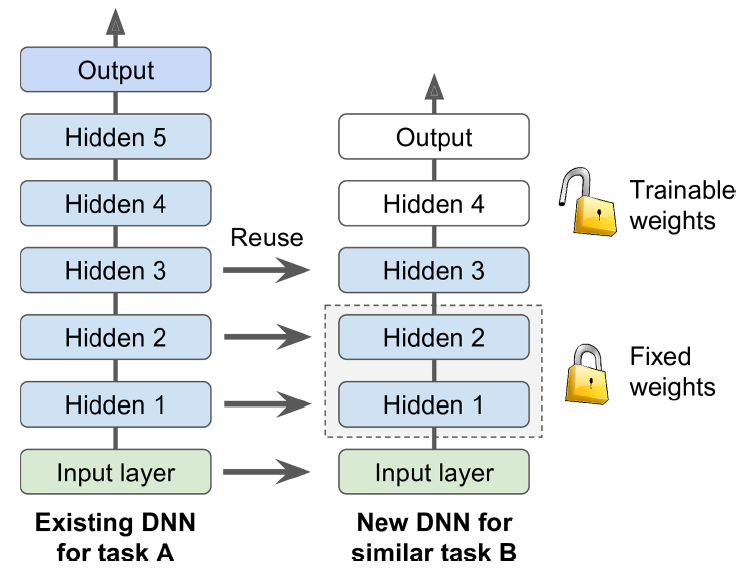
\includegraphics[width=0.70\textwidth]{2/figures/transfer_learning.PNG}
		\caption[Ejemplo de Transfer Learning]{Ejemplo de Transfer Learning. \\
		Fuente: \cite{bk_geron2022handml}. \textit{Hands-on machine learning with Scikit-Learn, Keras, and TensorFlow}.}
		\label{2:fig211}
	\end{center}
\end{figure}


\subsection{Arquitectura de Redes y Modelos Híbridos}
En los últimos años, el uso de arquitecturas híbridas que combinan Redes Neuronales Convolucionales (CNN) y Transformers de Visión (ViT) ha ganado popularidad debido a su capacidad para abordar tareas de clasificación de imágenes con mayor precisión. Estas arquitecturas híbridas aprovechan las fortalezas de ambas tecnologías: las CNNs son muy eficaces para extraer características locales en imágenes mediante filtros convolucionales, mientras que los ViTs permiten captar dependencias de largo alcance a través del mecanismo de auto-atención. La combinación de estas dos arquitecturas permite mejorar la clasificación de imágenes en ambientes no controlados, donde los datos pueden ser más complejos y menos estructurados.

\begin{figure}[H]
	\begin{center}
		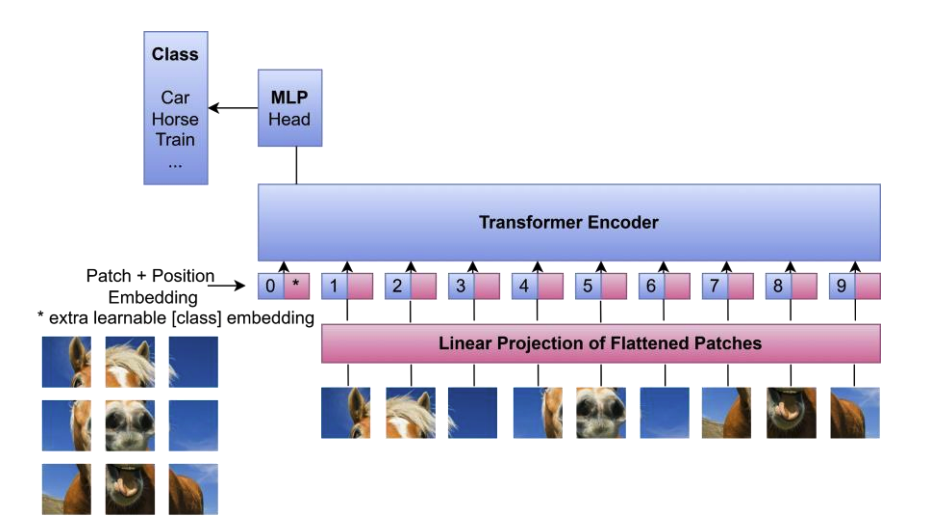
\includegraphics[width=0.70\textwidth]{2/figures/vit arquitechture.png}
		\caption[Arquitectura ViT]{Arquitectura ViT. \\
		Fuente: \cite{app13095521}. \textit{Comparing Vision Transformers and Convolutional Neural Networks for Image Classification: A Literature Review.}.}
		\label{2:fig211}
	\end{center}
\end{figure}


Los modelos híbridos, como CNN + ViT, combinan la robustez de las CNNs en la extracción de características visuales locales y la capacidad de los ViTs para manejar relaciones a largo plazo entre estas características. El uso de ViT ayuda a que el modelo sea más flexible frente a diferentes resoluciones de entrada, lo que es especialmente útil en contextos en los que las imágenes pueden variar en calidad y escala. Además, la arquitectura híbrida reduce la complejidad computacional en comparación con modelos puramente basados en ViT, al aprovechar la eficiencia de las CNNs en la etapa inicial del procesamiento de la imagen \parencite{yunusa2024exploringsynergieshybridcnns}.

\begin{figure}[H]
	\begin{center}
		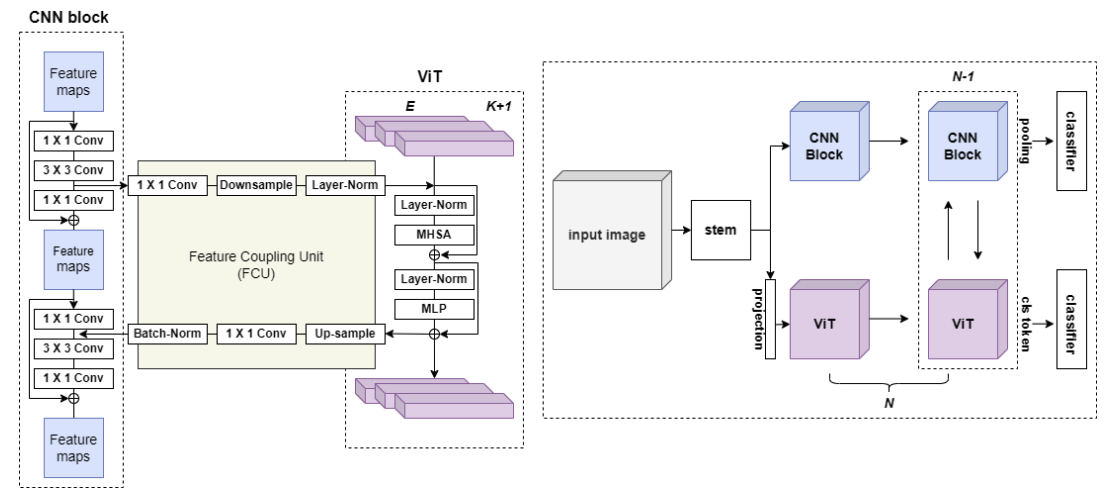
\includegraphics[width=0.70\textwidth]{2/figures/cnn+vitarquitechture.png}
		\caption[Conformer parallel integration of hybrid CNN and ViT]{Conformer parallel integration of hybrid CNN and ViT. \\
		Fuente: \cite{app13095521}. \textit{Comparing Vision Transformers and Convolutional Neural Networks for Image Classification: A Literature Review.}.}
		\label{2:fig211}
	\end{center}
\end{figure}



Un ejemplo destacado de esta tendencia es la combinación de CNNs con ViTs en tareas de clasificación de imágenes, donde se ha demostrado que la sinergia entre ambos modelos supera a los enfoques tradicionales basados únicamente en CNNs o ViTs. Esta combinación no solo mejora la precisión, sino que también incrementa la eficiencia del modelo al permitirle aprender tanto características locales como globales de las imágenes, un factor crucial cuando se trabaja con imágenes de pavimento en ambientes no controlados, como en el caso de la clasificación automatizada de deterioros en pavimentos \parencite{app13095521}.




\begin{comment}

\subsection{Ecografía y las imágenes de ultrasonido}
Según \cite{pr_herrera2017diseimp}, la ecografía, que es una técnica de diagnóstico en donde se usan imágenes generadas por ultrasonido, es comúnmente desarrollado en las áreas de cardiología, ginecología, y otras más relacionadas. La popularidad de esta técnica se basa en la capacidad de las imágenes de alta calidad que se obtienen de este proceso, además de no ser un método invasivo o de radiación como muchos otros de su tipo.

Los sistema encargados de extraer las imágenes de ultrasonido son compuestos de distintas sensores que generan ondas de sonido para posteriormente analizar la respuesta de la interacción física con el campo de interés. Estas señales recibidas de regreso son digitalizados por una parte electrónica delantera que también transforman estos datos crudos en la imagen final. El funcionamiento de este proceso depende de la configuración de los sensores, el método usado para obtener las imágenes y las características de área de interés. \parencite{pr_camacho2022ultrasonicimg}

Algunas imágenes de ultrasonido de nódulos tiroideos se muestran en la Figura \ref{2:fig210}.

\begin{figure}[H]
	\begin{center}
		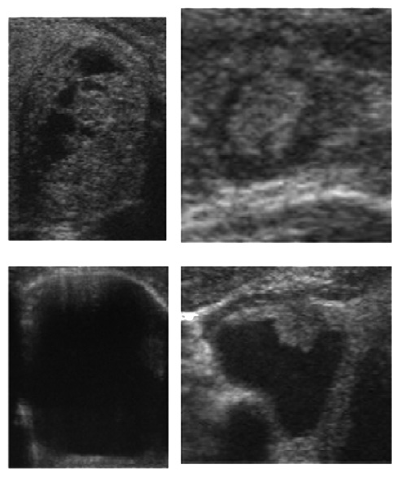
\includegraphics[width=0.40\textwidth]{2/figures/imagenes_ultrasonido_originales.png}
		\caption[Imágenes de ultrasonido de nódulos tiroideos]{Imágenes de ultrasonido de nódulos tiroideos. \\
		Fuente: \cite{pr_JERBI2023autoclassViTGAN}. \textit{Automatic classification of ultrasound thyroids images using vision transformers and generative adversarial networks}.}
		\label{2:fig210}
	\end{center}
\end{figure}




\subsection{Data Augmentation}

Según \cite{bk_geron2022handml} el Aumento de Datos o Data Augmentation es una técnica de regularización que permite reforzar la cantidad de muestras en un conjunto de datos. Esto se realiza a través de la generación de nuevas instancias similares a los originales; es decir, las personas no deberían ser capaces de diferenciar una imagen generada de una del propio conjunto de datos.

Para generar estas nuevas muestras, normalmente se aplican diferentes transformaciones a las instancias del conjunto de datos original. Estas transformaciones pueden ser; por ejemplo, una simple rotación o recorte de la imagen, siempre y cuando no altere por completo su sentido como es el caso de voltear una imagen de texto de forma horizontal. 

El principal beneficio de esta técnica es que permite reducir el sobreajuste de los modelos entrenados. 

En la Figura \ref{2:fig212} se muestran algunas transformaciones que se pueden hacer al aplicar el Aumento de Datos. 

\begin{figure}[H]
	\begin{center}
		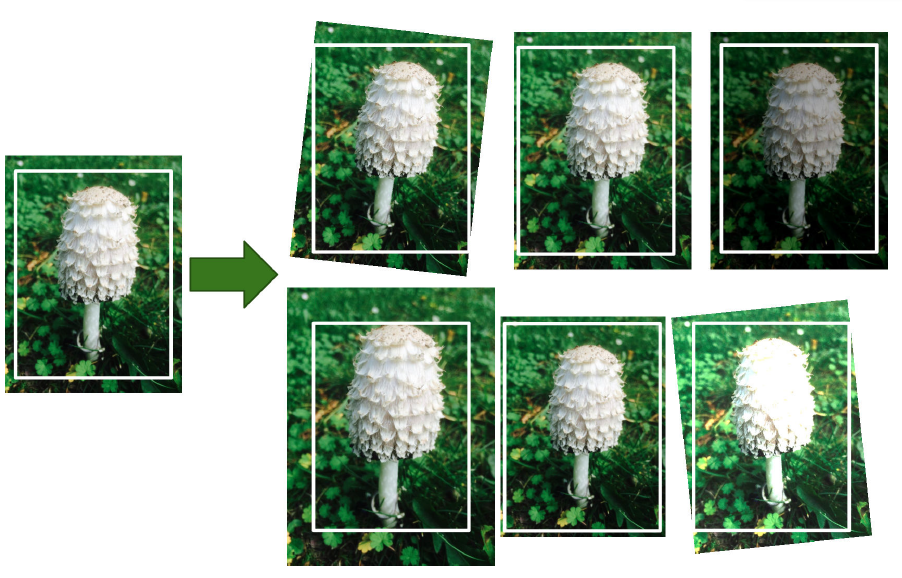
\includegraphics[width=0.85\textwidth]{2/figures/data_aug.PNG}
		\caption[Ejemplo de Data Augmentation]{Ejemplo de Data Augmentation. \\
		Fuente: \cite{bk_geron2022handml}. \textit{Hands-on machine learning with Scikit-Learn, Keras, and TensorFlow}.}
		\label{2:fig212}
	\end{center}
\end{figure}

\end{comment}